%=========================================================================================================================================
%=========================================================================================================================================
\chapter{Grundlagen (Beispiele f�r Formatierung)} \label{chapter:grundlagen}
%=========================================================================================================================================
%=========================================================================================================================================

Dieses Kapitel soll einen sanften Einstieg in den Bereich der Smartcards bieten. Aus diesem Grund wird zu Beginn dieser Arbeit auf die verschiedenen Hardwaretypen eingegangen. Da eine Chipkarte ohne Leseger�t wie der Fisch ohne Wasser ist, wird auch diese Hardwarekomponente behandelt. Um die Allgegenwart von Chipkarten zu veranschaulichen, wird schlussendlich ein Einblick in die Einsatzm�glichkeiten dieser Mini-Computer gegeben.

Informationen zu diesem Kapitel sind, wenn nicht anders angegeben, den beiden Standardwerken aus dem Bereich Chipkarten "`Handbuch der Chipkarten"' \cite{HandChip} und "`Chipkartenanwendungen"' \cite{ChipAnw} entnommen.

%-----------------------------------------------------------------------------------------------------------------------------------------
\section{Typen von Chipkarten}
%-----------------------------------------------------------------------------------------------------------------------------------------
Aufgrund der vielen Einsatzm�glichkeiten von Chipkarten, die mehr oder weniger Sicherheit \bzw mehr oder weniger Mobilit�t verlangen, kann man Chipkarten nach zwei Gesichtspunkten \gedankenstrich dem Chiptyp und der Daten�bertragung\gedankenstrich unterscheiden. Anhand des Chiptyps werden die Karten in Speicher- und Prozessorchipkarten unterteilt, wogegen sie durch die Daten�bertragung in kontaktbehaftete, kontaktlose und Dual-Interface \mbox{Karten} aufgegliedert werden.

Prozessorchipkarten haben im Unterschied zu Speicherchipkarten sehr viel st�rkere Sicherheitsma�nahmen implementiert und dienen als kleine Datentresore. Kontaktbehaftete Karten k�nnen nur von einem geeigneten Leseger�t mit Steckvorrichtung gelesen werden. Dagegen ist bei kontaktlosen Karten die Kommunikation nur �ber die Luftschnittstelle m�glich. Dual-Interface \mbox{Karten} sind eine Kombination aus diesen zwei Typen und beherrschen beide �bertragungstechniken. Diese Diplomarbeit besch�ftigt sich zum gr��ten Teil mit Prozessorchipkarten und geht auf Speicherchipkarten nur insoweit ein, um dem Leser den Unterschied zwischen diesen zu erkl�ren.

%Speicherchipkarten werden nur zur Vollst�ndigkeit erw�hnt.

%--------------------------------------------------------------------
\subsection{Speicherchipkarten}
%--------------------------------------------------------------------
Speicherchipkarten haben eine sehr einfache Logik, die es lediglich erlaubt, Daten in den Speicherbereich auf der Karte
zu schreiben und diese wieder zu lesen. Es sind sehr schwache Sicherheitsma�nahmen (\zb keine Erh�hung des Restbetrages
bei Wertkarten f�r Telefonzellen) zum Schutz der Daten vorhanden, wodurch sie f�r Hochsicherheits-Anwendungen
ungeeignet sind. Durch die geringen Sicherheitsanforderungen ben�tigen diese Karten auch keinen teuren (Co-)Prozessor.
Es sind lediglich EEPROM, ROM und eine Speicherverwaltung mit eventuell integrierter Sicherheitslogik notwendig.
Speicherchipkarten sind auch nicht derart stark \mbox{gegen} physikalische Angriffe gewappnet, wie das die hochwertigen
Prozessorkarten sind. Durch \mbox{dieses} einfache Design ist ihr Preis auch vergleichsweise gering. Ein schematischer
Aufbau ist in Abbildung \ref{fig:grundlagen:speicherkartenaufbau} dargestellt.
\begin{figure}[ht]
 \centering
 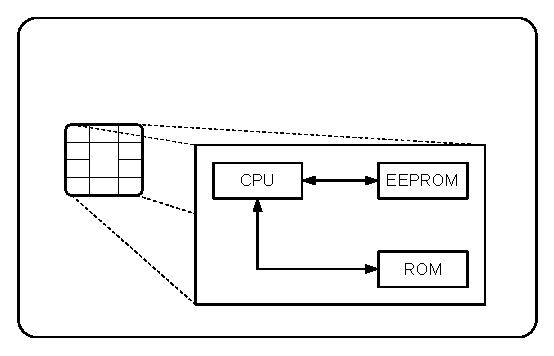
\includegraphics{grundlagen/speicherkarte}
 \figcaption{Prinzipieller Aufbau einer Speicherkarte}
 \label{fig:grundlagen:speicherkartenaufbau}
\end{figure}

%--------------------------------------------------------------------
\subsection{BER-TLV}
%--------------------------------------------------------------------
Die BER-TLV-Codierung (\engl basic encoding rule) wurde in der Norm ITU-T Rec. X.690 (siehe \cite{ITU:X.690}) definiert
und wird vom Standard \isostand{4} in leicht eingeschr�nkter Form �bernommen. Aufgrund der geringen Speicherf�higkeit
von Chipkarten wurde das maximale Fassungsverm�gen dieser Datenobjekte auf ein praktikables Ma� reduziert. Aufgrund der
TLV-Struktur besteht ein BER-TLV-Datenobjekt wiederum aus einem Kennzeichen, einer L�ngenangabe und dem optionalem
Nutzdatenteil (siehe Abbildung \ref{fig:smartcards:TLV:BER}).

%---------------------------------------
\subsubsection{Tag}
%---------------------------------------
Die Bezeichnung (siehe Tabelle \ref{fig:smartcards:tlv:bertlvbyteone1}) darf nach \isostand{4} eine L�nge von ein, zwei
oder drei Bytes besitzen. Dem ersten Byte kommt eine spezielle Bedeutung zu. Es ordnet das Datenobjekt (Bit 7 und 8) in
eine von vier Klassen ein.
\begin{enumerate}
\item \bin{00} bildet die universelle Klasse (\engl universal class)
\item \bin{01} bildet die Applikationsklasse (\engl application class)
\item \bin{10} bildet die kontext-spezifische Klasse (\engl context-specific class)
\item \bin{11} bildet die private Klasse (\engl private class)
\end{enumerate}

\ArialTable{Codierung des ersten Kennzeichenbytes nach dem BER-TLV-Schema}{fig:smartcards:tlv:bertlvbyteone1} {
\begin{tabularx}{\linewidth}{|cc|c|ccccc|X|} \hline \rowcolor{Gray}
  b8 & b7 & b6 & b5 & b4 & b3 & b2 & b1 & Bedeutung                           \\ \hline
   0 &  0 &  - &  - &  - &  - &  - &  - & universelle Klasse                  \\
   0 &  1 &  - &  - &  - &  - &  - &  - & Applikationsklasse                  \\
   1 &  0 &  - &  - &  - &  - &  - &  - & kontext-spezifische Klasse          \\
   1 &  1 &  - &  - &  - &  - &  - &  - & private Klasse                      \\ \hline
   - &  - &  0 &  - &  - &  - &  - &  - & einfach (\engl primitiv)            \\
   - &  - &  1 &  - &  - &  - &  - &  - & zusammengesetzt (\engl constructed) \\ \hline
   - &  - &  - &  x &  x &  x &  x &  x & einfaches Kennzeichen               \\
   - &  - &  - &  1 &  1 &  1 &  1 &  1 & komplexes Kennzeichen               \\ \hline
\end{tabularx}}
%-----------------------------------------------------------------------------------------------------------------------------------------
\section{Kein 1.1 ohne 1.2}
%-----------------------------------------------------------------------------------------------------------------------------------------

\vspace*{13cm}
Keine Leerseiten!
\newpage

%-----------------------------------------------------------------------------------------------------------------------------------------
\section{Keine mehrzeiligen �berschriften; das sieht schrecklich aus und l�sst sich immer vermeiden!}
%-----------------------------------------------------------------------------------------------------------------------------------------

%-----------------------------------------------------------------------------------------------------------------------------------------
\section{Keine mehrzeiligen �berschriften}
%-----------------------------------------------------------------------------------------------------------------------------------------
Das sieht schrecklich aus und l�sst sich immer vermeiden!

\vspace*{8cm}
\begin{itemize}
  \item Leerr�ume nur am Kapitelende!
  \item Auch die letzte Seite sollte mindestens zur H�lfte gef�llt sein!
\end{itemize}
\newpage

\cleardoublepage
%=========================================================================================================================================
%=========================================================================================================================================
% EOF
%=========================================================================================================================================
%=========================================================================================================================================
